\begin{titlepage}
	\newgeometry{left=0cm, right=0cm, top=0cm, bottom=0cm}
	\begin{tikzpicture}[ultra thick]
	\shade [top color=CadetBlue!70!green, bottom color=CadetBlue!80!green] (0,0) rectangle (\textwidth,\textheight);
	\filldraw[fill=DarkCyan!70!DarkGreen, draw=gray!30, ultra thick, rounded corners=1cm] (4,17) rectangle (\textwidth + 1cm, 25);
	\node [text width = 13cm, align=left, text=white] at (13,21) {\Huge Physical Computing \\\huge Eine Einführung in Informatik und Physik des Arduino mit dem Open Roberta Lab \\ \vspace{1cm} \huge Sebastian Voß};
	\node [inner sep=0mm] at (7,11) {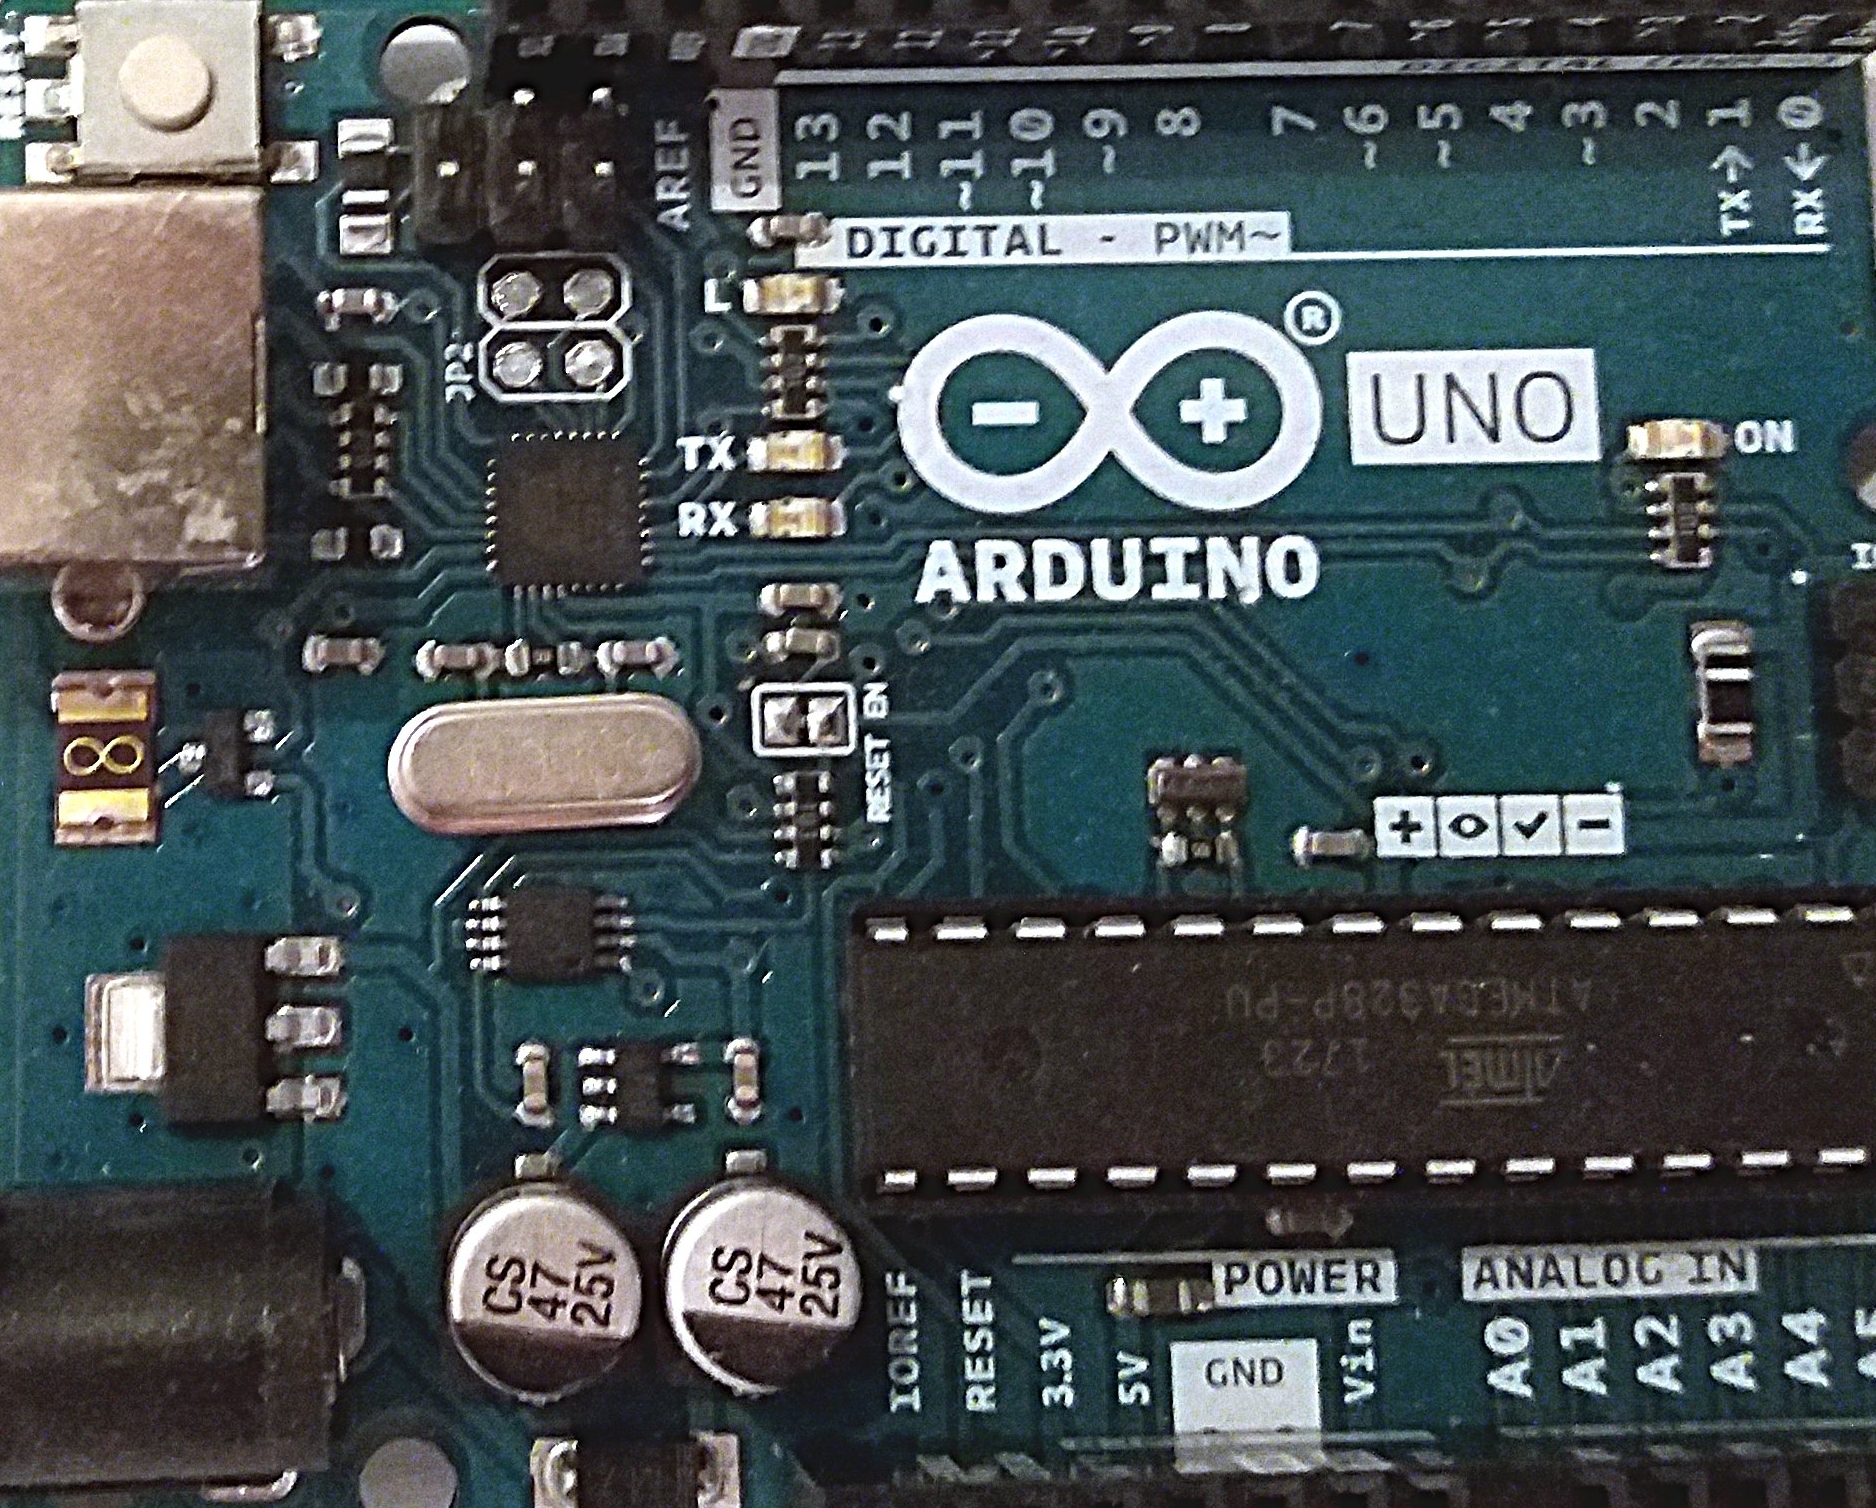
\includegraphics[width=.4\textwidth, angle=35]{./pics/arduino-titel.jpg}};
	\node [inner sep=0mm] at (15,5) {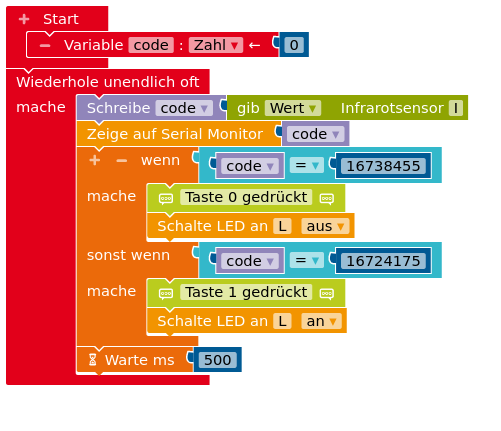
\includegraphics[width=.5\textwidth]{./pics/ir-fernbedienung-auslesen.png}};
	%  LED
	\draw [rotate around={-15:(5,8)}, color=yellow] (14,17) -- ++(1,0) ++(0,0.5) -- ++(0,-1) -- ++(1,0.5) ++(-1,0.5) -- ++(1,-0.5) ++(0,0.5) -- ++(0,-1) ++ (0,0.5) -- ++(1,0);
	\draw [->, color=yellow, rotate around={-15:(5,8)}] (14,17) ++(1.2,0.5) -- ++(0.2,0.4);
	\draw [->, color=yellow, rotate around={-15:(5,8)}] (14,17) ++(1.5,0.5) -- ++(0.2,0.4);
	% Widerstand
	\draw [rotate around={90:(2,15)}, color=red!80!black] (2,15) -- ++(1,0) ++(0,-0.5) rectangle ++(2,1) ++(0,-0.5) -- ++(1,0);
	%  LDR
	\draw [color=blue!80!black] (11,27) -- ++(1,0) ++(0,-0.5) rectangle ++(2,1) ++(0,-0.5) -- ++(1,0);
	\draw [color=blue!80!black, <-] (11,27) ++(2,0.6) -- ++(-0.2,0.4);
	\draw [color=blue!80!black, <-] (11,27) ++(1.7,0.6) -- ++(-0.2,0.4);
	\draw [color=blue!80!black, ->] (11,27) ++(1.1,-0.7) -- ++(0.3,0) -- ++(1.6,1.6);
	% Motor
	\draw [rotate around={-30:(2,4)}, color=magenta!80!black] (2,4) -- ++(1,0) ++(0.5,0) circle [radius=0.5cm] node {\huge \bfseries \sffamily M} ++(0.5,0) -- ++(1,0);
	% Transistor
	\draw [rotate around={20:(3,26)}, color=yellow!50!red] (3,26) -- ++(0.5,0) -- ++(0.2,-0.4) -- ++(0.2,0) -- ++(0,-0.4) ++(0,0.4) -- ++(0.2,0) -- ++(0.2,0.4) -- ++(0.5,0) ++(-0.9,-0.05) circle [radius=0.5cm];
	\draw [rotate around={20:(3,26)}, color=yellow!50!red,->] (3,26) ++(1.1,-0.4) -- ++(0.15,0.3);
	\end{tikzpicture}
\end{titlepage}